\chapter{Numerical model for vegetation in urban areas}
\label{ch:numericalmethod}
\def\figdir{chapters/ch07_numericalmodel/figures}	

\section{Introduction}

In this chapter, the numerical method for modeling vegetation inside an urban area is described. The numerical model consists of air domain model (\cref{sec:airdomain}), solid domain model (\cref{sec:soliddomain}) and the radiation model \cref{sec:radiationmodel}. \cref{fig:fullmodelcoupling} shows the coupling between these three models and the parameters that are communicated between them. A detailed description of the coupling algorithm is provided in \cref{sec:couplingalgorithm}. 

\begin{figure}[h]
	\centering
	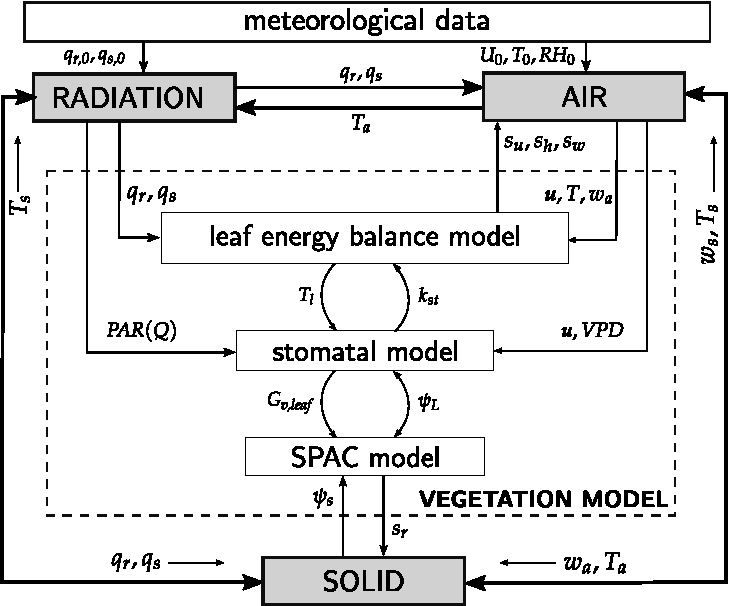
\includegraphics[width=\textwidth]{\figdir/fullmodelcoupling-crop.pdf}
	\caption{Coupling of the vegetation model with air domain solver, solid domain solver and the radiation model. The indicated parameters are used for coupling the methods. }
	\label{fig:fullmodelcoupling}
\end{figure}

The air domain model describes the transport of moist air through vegetation (i.e., velocity $\mvec{u}$, enthalpy $h$, moisture content $w_a$, and CO$_2$ concentration $x_c$). Furthermore, with the air domain, the \textit{leaf energy balance} (LEB) model is solved to determine the heat and mass fluxes (i.e., $q_{\textit{sen,leaf}}$ and $g_{\textit{v,leaf}}$). A detailed description of the leaf energy balance is provided in \cref{ch:parametricstudy}. The solid domain model described the coupled heat and mass transport (i.e., $T_s$, and $w_s$) in all urban materials (i.e. ground, pavement, and building facades). Furthermore, the soil ground domain which consists of vegetation roots, additionally solves the \textit{soil-plant-atmosphere continuum} (SPAC) model to determine the root water uptake $g_{\textit{v,root}}$ in the soil and the leaf water potential $\psi_L$ (see \cref{sec:spac}). Finally, the radiation model determines the short-wave $q_s$ and long-wave $q_r$ radiative exchanges in the urban street canyon including the impact of vegetation (see \cref{sec:radiationmodel}). 

\section{Air domain: Transport of moist air}
\label{sec:airdomain}
The simplified vegetation model is described in \cref{ch:parametricstudy}, introduction the governing equation for moist flow through vegetation. The vegetation model, consisting of the ``\textit{leaf energy balance}'' (LEB) model, provides the necessary source/sink terms for heat, mass and momentum exchanges between vegetation and air as described in \cref{sec:cons_incompressible}. For reader, a detailed derivation of the thermodynamic of the moist air is given in \cref{app:thermodynamics} and a detailed derivation of the governing equation of moist flow is given in \cref{app:conservation}. In this section, we summarize the pseudo-compressible form of governing equation for moist flow through vegetation where the buoyancy force is directly obtained from the density field.  

\subsection*{Conservation of mass}

The governing equation consists of conservation of mass, momentum, energy and species. The conservation equations are given in differential form in a Cartesian coordinate system described by the triplet $\mvec{x} = (x,y,z)$. The conservation of mass for compressible moist flow is given as:
\begin{equation}
\frac{\partial \rho}{\partial t} + \nabla \cdot \left( \rho \mvec{u} \right)= 0
\end{equation}
where $\rho$ is the fluid density (kg\,m$^{-3}$), and $\mvec{u} = \left(u,v,w\right)$ is the fluid velocity (m\,s$^{-1}$). A detailed derivation is given in appendix \ref{app:thermodynamics} and \ref{app:conservation}.

\subsection*{Conservation of momentum}

The conservation of momentum is given as:
\begin{equation}
\frac{\partial \rho \mvec{u}}{\partial t} + \nabla  \cdot \left( \rho \mvec{u} \mvec{u} \right) = -\nabla p + \mu \nabla^2 \mvec{u} + \rho \mvec{g} + \mvec{s}_u
\end{equation}
where $p$ is the pressure (Pa), $\mu$ the dynamic viscosity (kg\,m$^{-1}$\,s$^{-1}$), $\mvec{g}$ the gravitational acceleration (m\,s$^{-2}$). The source of momentum $\mvec{s}_u$ is:
\begin{equation}
\mvec{s}_u = - \rho a c_d |\mvec{u}|\mvec{u}
\end{equation}
where $a$ is the leaf area density (m$^2$\,m$^{-3}$), and $c_d$ is the leaf drag coefficient ($c_d = 0.2$).

\subsection*{Conservation of energy}

The conservation of energy is given as:
\begin{equation}
\frac{\partial \rho h}{\partial t} + \nabla  \cdot \left( \rho h \mvec{u} \right) = -\nabla \cdot \mvec{q} + s_h
\end{equation}
where 
\begin{equation}
\mvec{q} = - \lambda \nabla T
\end{equation}
is the Fourier's law of heat conduction, with:
\begin{equation}
\mvec{q} = - \frac{c_p \mu}{\mathrm{Pr}} \nabla T
\end{equation}
and the source of energy $s_h$ is 
\begin{equation}
\mvec{s}_h = \rho c_p a q_{\textit{sen,leaf}}
\end{equation}

\subsection*{Conservation of species}

In our study, the species of interest is water vapor (subscript $v$) and carbon-dioxide (subscript $c$). The conservation of species $i$ is given as:
\begin{equation}
\frac{\partial \rho x_i}{\partial t} + \nabla  \cdot \left( \rho x_i \mvec{u} \right) = \nabla \cdot \mvec{g}_i + s_i
\end{equation}
where $x_i$ is the concentration of species $i$, $\mvec{g}_i$ is the flux of species, and $s_i$ is the source term. 

We assume that moist air is composed of dry air and water vapor. The mass fraction of each component is:
\begin{equation}
x_a = \frac{\rho_a}{\rho}
\end{equation}
and
\begin{equation}
x_v = \frac{\rho_v}{\rho}
\end{equation}
where $\rho_a$ and $\rho_v$ are partial density of dry air and water vapor (kg\,m$^{-3}$) and $\rho$ is density of gas mixture and results in:
\begin{equation}
x_a + x_v = 1
\end{equation}
and
\begin{equation}
\rho_a + \rho_v = \rho
\end{equation}

The enthalphy of dry air and water vapor are:
\begin{equation}
h_a = c_{p,a} \left(T - T_{\mathit{ref}}\right)
\end{equation}
and
\begin{equation}
h_v = c_{p,v} \left(T - T_{\mathit{ref}}\right) + L_v \left(x_v - x_{v,ref}\right)
\end{equation}

The total enthalpy of moist air is:
\begin{equation}
h = h_a \, x_a + h_v \, x_v
\end{equation}
and so:
\begin{equation}
\rho h = \rho_a c_{p,a} \left(T - T_{\mathit{ref}}\right) + \rho_v c_{p,v} \left(T - T_{\mathit{ref}}\right) + \rho_v L_v
\end{equation}

\subsection*{Turbulence modeling}

The Reynolds decomposition splits the instantaneous velocity into mean and fluctuating component:
\begin{equation}
\mvec{u} \left(\mvec{x},t\right) = \overline{\mvec{u}} \left(\mvec{x}\right) + \mvec{u}' \left(\mvec{x},t\right).
\end{equation}

Applying this averaging operator to the NS equations, resulting Reynolds-Averaged Navier-Stokes (RANS) equation is given as:
\begin{equation}
\frac{\partial \overline{\rho}}{\partial t} + \nabla \cdot \left(\overline{\rho}\,\overline{\mvec{u}}\right) = 0,
\end{equation}
\begin{equation}
\frac{\partial \overline{\rho}\,\overline{\mvec{u}}}{\partial t}  + \nabla \cdot \left(\overline{\rho}\,\overline{\mvec{u}}\,\overline{\mvec{u}}\right) = -\nabla \overline{p} + \mu \nabla^2 \overline{\mvec{u}} - \nabla \cdot \left(\overline{\rho \mvec{u}' \mvec{u}'}\right)+ \rho \mvec{g} + s_u
\end{equation}
where $\overline{\rho \mvec{u}' \mvec{u}'}$ is the Reynolds stresses. The Reynolds stresses are modelled using Bousinessq eddy-viscosity assumption:
\begin{equation}
- \overline{\rho \mvec{u}' \mvec{u}'} = \mu_t \left(\nabla u + \nabla u^T\right) - \frac{2}{3}\rho k \mvec{I}
\end{equation}
where:
\begin{equation}
\mu_t = \rho C_\mu \frac{k^2}{\varepsilon}
\end{equation}


\section{Solid domain: Coupled heat and moisture transport}
\label{sec:soliddomain}
\subsection{Composition of the porous material}

The building materials and the soil is considered as a porous material consisting of three phases: solid phase (denoted with $s$), liquid phase referring to liquid water ($l$) and the air phase which is split into dry air ($a$) and water vapor $v$ \citep{Defraeye2011, Saneinejad2013, Carmeliet2005,Janssen2002}. The open porosity $\phi_o$ (m$^3$\,m$^{-3}$) of the porous material is defined as:
\begin{equation}
\phi_o = \frac{V_{\mathit{pore}}}{V}
\end{equation}
where $V_{\textit{pore}}$ (m$^3$) is the volume of open pores and $V$ (m$^3$) is the total volume of the porous material $\tensor{S}$. The solid material content $w_s$ (kg\,m$^{-3}$) is defined as:
\begin{equation}
w_s = \left(1 - \phi_o \right) \rho_s
\end{equation}
where $\rho_s$ (kg\,m$^{-3}$) is the solid material matrix density. Similarly the dry air $w_a$, water vapor $w_v$, liquid water $w_l$ contents are defined as:
\begin{align}
w_l &= \phi_o S_l \rho_l \\
w_a &= \phi_o \left( 1 - S_l \right) \rho_a \\
w_v &= \phi_o \left( 1 - S_l \right) \rho_v
\end{align}
where they are related to the degree of liquid saturation $S_l$ of the porous open pores:
\begin{equation}
S_l = \frac{\phi_{\textit{o,l}}}{\phi_o}
\end{equation}
with $\phi_{\textit{o,l}}$ being the amount of liquid water occupied inside the open pores and $\rho_a$, $\rho_l$ being the air and liquid water densities, respectively. The total moisture content $w$ (kg\,m$^{-3}$) inside the porous material is simply the sum of liquid water and water vapor:
\begin{equation}
w = w_l + w_v
\end{equation}

\subsection{Water potential}

Water potential is a universal parameter to determine the \textit{water status} in any medium \citep{nobel2009physicochemical}. In the thesis, we use it to define the water status of multiple domains such as solid porous materials (soil and building facades), plant xylem, and air. The water potential $\psi$ (Pa) describes the chemical potential of water $\mu$ (J\,mol$^{-1}$) with respect to chemical potential of pure water $\mu^{o,l}$ (J\,mol$^{-1}$) at the same temperature, standard atmosphere and at zero level:
\begin{equation}
\psi = \frac{\mu - \mu^{o,l}}{V^o_l}
\end{equation}
where $V^o_l = 18.05 \num{e-3}$ m$^3$\,mol$^{-1}$ is the molar volume of pure water in liquid phase. The water potential for pure water at standard atmosphere is $\psi = 0$ Pa. The water tends to move towards a region where $\mu-\mu^{o_w}$ is lower, i.e. in the direction of $-\nabla\psi$. The water potential is related to pressure potential, osmotic potential, matrix potential, and gravitational potential. In our study, we assume that the pressure potential gradient is negligible in the solid and we ignore the influence of osmotic potential $\psi_o$ (Pa) as we assume we have a non-saline porous material. Therefore, only the matrix potential and gravitation potential influences the water transport:
\begin{equation}
\psi = \underbrace{p_c}_{\psi_c} + \underbrace{\rho_l g z}_{\psi_g}
\end{equation}
where $\psi_c = p_c$ (Pa) is the capillary potential due to capillary pressure, which represents the contribution of the matrix potential, and $\psi_g = \rho_l g h$ (Pa) is the gravitational potential with $g = |\mvec{g}|$ (m\,s$^{-2}$) where $\mvec{g}$ is the gravitational acceleration. The capillary pressure $p_c$ is defined as the difference between liquid and gas phase pressure, $p_l$ and $p_g$, respectively:
\begin{equation}
p_c =  p_l - p_g
\end{equation}
and is related to relative humidity $\phi$ by the Kelvin's law:
\begin{equation}
p_c = \rho_l R_v T \ln \left(\phi\right)
\end{equation}

The gravitational potential $\psi_g$ (Pa) is defined as:
\begin{equation}
\psi_g = - \rho \mvec{g} \cdot \mvec{x} = \rho g z
\end{equation}
where $g = |\mvec{g}|$ with $z$ oriented upward. Thus, by taking the capillary and gravitational water potentials into account, the transport of water can be described in building materials and, more importantly, soil where the plant roots are present.

\subsection{Coupled transport of heat and mass}
\label{subsec:ctoham}
\subsubsection*{Conservation of mass}
The conservation of mass in the solid domain is defined as:
\begin{align}
\pde{w_s}{t} &= 0 \label{eq:solidcom} \\ 
\pde{w_a}{t} + \nabla \cdot \left(w_a\mvec{u}_a \right) &= 0 \label{eq:aircom} \\ 
\pde{w_l + w_v}{t} + \nabla \cdot \left(w_l\mvec{u}_l + w_v\mvec{u}_v \right) &= 0 \label{eq:liqcom}
\end{align}
assuming that solid matrix does not move, mass of different phases only change due to evaporation or condensation. Other phenomena such as melting, freezing, sublimation and deposition are neglected. Assuming dry air does not contribute to moisture storage, i.e., $\partial w_a / \partial t = 0$, the conservation of mass simplifies to rate of change of moisture content $w = w_l + w_v$, from \cref{eq:liqcom}:
\begin{equation}
 \pde{w}{t} = - \nabla \cdot \left(\mvec{g}_l + \mvec{g}_v \right)
\end{equation}
where $\mvec{g}_l \equiv w_l\mvec{u}_l$ (kg\,m$^{-2}$\,s$^{-1}$) and $\mvec{g}_v \equiv w_v\mvec{u}_v$ (kg\,m$^{-2}$\,s$^{-1}$) are defined as the liquid water and water vapor fluxes, respectively. Additionally, the contribution of root water uptake due to plant transpiration is introduced through the source term $s_r$ (kg\,m$^{-3}$\,s$^{-1}$):
\begin{equation}
\pde{w}{t} = - \nabla \cdot \left(\mvec{g}_l + \mvec{g}_v \right) + s_r
\label{eq:com4}
\end{equation}

The sink term due to root water uptake is explained in detail later in \cref{sec:spac}. In this thesis, the conservation of mass is solved using the $p_c$-form Richards equation, where \cref{eq:com4} becomes:
\begin{equation}
\frac{\partial w}{\partial p_c} \frac{\partial p_c}{\partial t} = -  \nabla \cdot \left(\mvec{g}_l + \mvec{g}_v\right) + s_{r}
\label{eq:com5}
\end{equation}
with $C_{mm} \equiv \partial w/ \partial p_c$ (kg\,m$^{-3}$\,Pa$^{-1}$) is defined as the moisture capacity. Thus, the change in water content in the porous material is simply due to the liquid and vapor fluxes, and root water uptake. The liquid water flux $\mvec{g}_l$ in porous media is given by:
\begin{equation}
\mvec{g}_l = - K_{\textit{lp}} \nabla \left(p_c + \rho_l g z\right)
\label{eq:liquidflux}
\end{equation}
and assumes the air pressure effects be negligible with respect to capillary and gravitational effects, where $K_{\textit{lp}}$ (s) the liquid water permeability. We assume that the liquid water permeability is only due to pressure gradient, and the influence of thermal gradient is neglected \citep{Carmeliet2005}. The water vapor flux in the porous media is given by:
\begin{equation}
\mvec{g}_v = K_{\textit{vp}}\nabla p_c + K_{\textit{vT}}\nabla T
\label{eq:vaporflux}
\end{equation}
where
\begin{equation}
K_{\textit{vp}} = - \delta_v \frac{p_v}{\rho_l R_v T}
\end{equation}
is the water vapor permeability (s) due to pressure,  
\begin{equation}
K_{\textit{vT}} = - \delta_v \frac{p_v}{\rho_l R_v T^2}\left(\rho_l L_v - p_c\right)
\end{equation}
is the water vapor permeability (s) due to temperature, and
\begin{equation}
\delta_v = \frac{D_{\textit{va,mat}}}{R_v T}
\end{equation}
is the water vapor diffusion coefficient (s) where $D_{\textit{va,mat}}$ (m$^2$\,s$^{-1}$) is the binary apparent diffusion coefficient between dry air and water vapor \citep{Carmeliet2005, Defraeye2011, Saneinejad2013, Kubilay2014b}. Thus, substituting the fluxes \cref{eq:liquidflux,eq:vaporflux} into \cref{eq:com5}, the expanded form of conservation of mass is given as:
\begin{equation}
C_{\textit{mm}}\frac{\partial p_c}{\partial t} = \nabla \cdot \Big( K_{lp} \nabla \left(p_c + \rho_l g z\right) + K_{\textit{vp}}\nabla p_c + K_{\textit{vT}}\nabla T \Big) + s_r
\label{eq:com6}
\end{equation}

\subsubsection*{Conservation of energy}
The conservation of energy is given as:
\begin{equation}
\frac{\partial h}{\partial t} + \nabla \cdot \left(h \mvec{u}\right) = - \nabla \cdot \mvec{q}
\label{eq:coe1}
\end{equation}
where $h$ (J\,kg$^{-1}$) is the enthalpy of total solid domain:
\begin{equation}
h = \sum_i w_i h_i = w_s h_s + w_a h_a + w_l h_l + w_v h_v
\label{eq:enthalphy1}
\end{equation}
and heat conduction $\mvec{q}$ (W\,m$^{-2}$) is given by Fourier's law as:
\begin{equation}
\mvec{q} = -\lambda \nabla T
\label{eq:fourierlaw}
\end{equation}
where $T$ (K) is temperature, $\lambda$ (W\,m$^{-1}$\,K$^{-1}$) is thermal conductivity.

Substituting \cref{eq:enthalphy1} into \cref{eq:coe1} expands to:
\begin{equation}
\frac{\partial}{\partial t}\left(w_s h_s + w_a h_a + w_l h_l + w_v h_v \right) + \nabla \cdot \left(w_a \mvec{g}_a + w_l \mvec{g}_l + w_v \mvec{g}_v\right) = - \nabla \cdot \mvec{q}
\label{eq:coe1p1}
\end{equation}
and assuming dry air and water vapor does not contribute to heat storage, i.e., $\partial w_a h_a / \partial t \approx 0$ and $\partial w_v h_v / \partial t \approx 0$, and convection term of dry air is negligible $\nabla \cdot w_a \mvec{g}_a \approx 0$, \cref{eq:coe1p1} simplified to:
\begin{equation}
\frac{\partial \left(w_s h_s + w_l h_l \right)}{\partial t} + \nabla \cdot \left(w_l \mvec{g}_l + w_v \mvec{g}_v\right) = - \nabla \cdot \mvec{q}
\label{eq:coe1p2}
\end{equation}

The enthalpies of solid $h_s$, liquid water $h_l$ and water vapor $h_v$ are defined as:
\begin{align}
h_s &= c_{ps} \left(T - T_{\textit{ref}}\right) \label{eq:enthalphys}\\
h_l &= c_{pl} \left(T - T_{\textit{ref}}\right) \label{eq:enthalphyl}\\
h_v &= c_{pv} \left(T - T_{\textit{ref}}\right) + L_v \label{eq:enthalphyv}
\end{align}
and $L_v$ is the latent heat of vaporization of water. Substituting \cref{eq:enthalphys,eq:enthalphyl,eq:enthalphyv} into \cref{eq:coe1p2}, the conservation of energy is given as:
\begin{equation}
\begin{split}
&\left(c_{\textit{ps}} w_s + c_{\textit{pl}} w\right)\frac{\partial T}{\partial t} + \left[c_{pl} \left(T - T_{\textit{ref}}\right) \frac{\partial w}{p_c}\right]\frac{\partial p_c}{\partial t} =\\
& - \nabla \cdot \bigg\{ {\mvec{q} + \underbrace{ c_{\textit{pl}} \left(T - T_{\textit{ref}}\right)\mvec{g}_l}_{\mvec{q}_l} + \underbrace{ \Big[c_{\textit{pv}} \left(T - T_{\textit{ref}}\right) + L_v\Big]\mvec{g}_v}_{\mvec{q}_v} } \bigg\}
\end{split}
\label{eq:coe3}
\end{equation}
where:
\begin{align}
C_{\textit{TT}} &=  c_{\textit{ps}}w_s + c_{\textit{pl}}w \label{eq:cap1} \\
C_{\textit{Tp}} &=  c_{\textit{pl}} \left( T - T_{\mathit{ref}}\right) \pde{w}{p_c} \label{eq:cap2} 
\end{align}
are the thermal capacity terms. Substituting liquid and vapour fluxes, \cref{eq:liquidflux,eq:vaporflux}, respectively, thermal capacities \cref{eq:cap1,eq:cap2} and heat conduction \cref{eq:fourierlaw} into conservation of energy expands \cref{eq:coe3} to:
\begin{align}
\begin{aligned}
		\mathllap{C_{\textit{TT}}\frac{\partial T}{\partial t} + C_{\textit{Tp}}\frac{\partial p_c}{\partial t}} = \nabla \cdot \bigg(\lambda \nabla T &+  K_{\textit{lp}} c_{\textit{pl}} \left(T - T_{\textit{ref}}\right)  \nabla p_c \\
					&+ K_{\textit{lp}} c_{\textit{pl}} \left(T - T_{\textit{ref}}\right) \rho_l g z\\
					&- K_{\textit{vp}} \Big[c_{\textit{pv}} \left(T - T_{\textit{ref}}\right) + L_v\Big] \nabla p_c \\ 
					&- K_{\textit{vT}} \Big[c_{\textit{pv}} \left(T - T_{\textit{ref}}\right) + L_v\Big] \nabla T \bigg)
\end{aligned}
\end{align}

\subsection{Linearized heat and mass transport equation}

In the present study, the conservation of mass and energy is coupled together as a heat and mass model (HAM) according to \citep{Janssen2002,Defraeye2011,Carmeliet2005,Saneinejad2013,Kubilay2018}. Due to the shape of the water retention curve and the hydraulic conductivity curve, as shown in\cref{fig:wrc}, the Richards equation is highly non-linear. Therefore, the numerical solution of the equation is very sensitive to convergence tolerance and requires linearization techniques to maintain accuracy and computational efficiency. So, methods such as fixed-point Picard iterations is used to solve the non-linear equations. More details on the discretization is provided in \cite{Liu2012,Janssen2002,Kubilay2018}. 

The conservation of mass (i.e., the moisture transport equation), \cref{eq:com6}, in the linearized form is given as:
\begin{equation}
\begin{split}
C^{n+1,k}_{\textit{mm}}\frac{p_c^{n+1,k+1}-p_c^{n}}{\Delta t} = \nabla \cdot \Big( K_{\textit{lp}}^{n+1,k} &\nabla \left(p_c^{n+1,k+1} + \rho_l g z\right)\\
&+ K_{\textit{vp}}^{n+1,k} \nabla p_c^{n+1,k+1} \\
&+ K_{vT}^{n+1,k} \nabla T^{n+1,k}\Big)\\
+ s_r^{n+1,k+1}&
\end{split}
\end{equation}
where the capacity, permeabilities and temperature are determined from the previous Picard iteration ($k$). The subscript ($n$) denotes the global (i.e., outer) time step of $t$ and $k$ denoting the internal Picard iteration step. When the Picard solution approaches convergence, i.e., $p_c^{n+1,k} \rightarrow p_c^{n+1,k+1}$, $\partial{w}/\partial p_c$ becomes negligible resulting in larger mass conservation errors. The error is minimized by formulating the Richard's equation in mixed-form \citep{Liu2012}:
\begin{equation}
\begin{split}
C^{n+1,k}_{\textit{mm}}\frac{p_c^{n+1,k+1}-p_c^{n}}{\Delta t} = \nabla \cdot \Big( K_{\textit{lp}}^{n+1,k} &\nabla \left(p_c^{n+1,k+1} + \rho_l g z\right)\\
&+ K_{\textit{vp}}^{n+1,k} \nabla p_c^{n+1,k+1} \\
&+ K_{vT}^{n+1,k} \nabla T^{n+1,k}\Big)\\
+ s_r^{n+1,k+1} &- \frac{w^{n+1,k+1}-w^n}{\Delta t}
\end{split}
\end{equation}
where an additional moisture change term is added.

\begin{figure}[t]
	\centering
	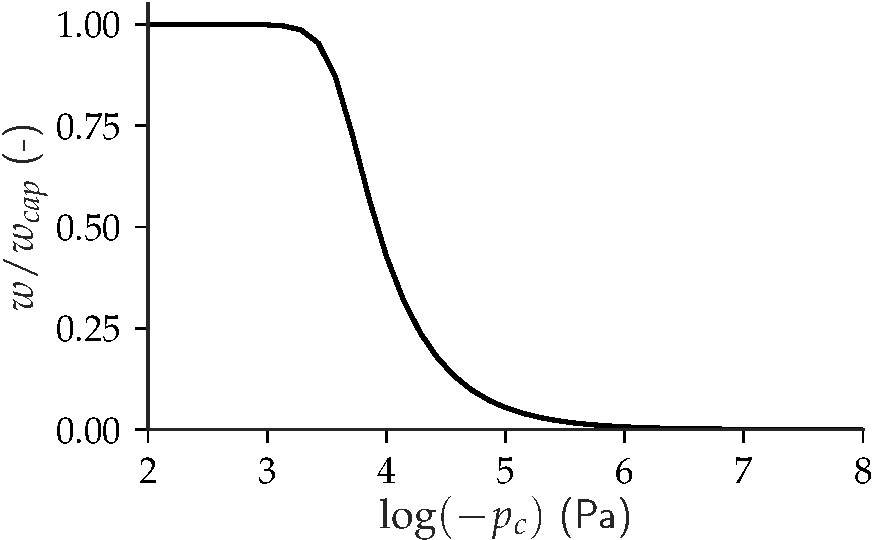
\includegraphics[width=0.5\textwidth]{\figdir/waterretentioncurve-crop.pdf}
	\caption{Typical non-linear moisture water retention curve for a material which is capillary saturated.}
	\label{fig:wrc}
\end{figure}

The linearized form of the heat equation is given as:
\begin{equation}
\begin{split}
	C_{\textit{TT}}^{n+1,k}& \frac{T^{n+1,k+1}-T^{n}}{\Delta t} = \nabla \cdot \bigg(\lambda \nabla T^{n+1,k+1} \\
	&+ K_{\textit{lp}}^{n+1,k} c_{\textit{pl}} \left(T^{n+1,k+1} - T_{\textit{ref}}\right)  \nabla p_c^{n+1,k+1} \\
	&+ K_{\textit{lp}}^{n+1,k} c_{\textit{pl}} \left(T^{n+1,k+1} - T_{\textit{ref}}\right) \rho_l g z\\
	&- K_{\textit{vp}}^{n+1,k} \Big[c_{\textit{pv}} \left(T^{n+1,k+1} - T_{\textit{ref}}\right) + L_v\Big] \nabla p_c^{n+1,k} \\ 
	&- K_{\textit{vT}}^{n+1,k} \Big[c_{\textit{pv}} \left(T^{n+1,k+1} - T_{\textit{ref}}\right) + L_v\Big] \nabla T^{n+1,k+1} \bigg)
\end{split}
\end{equation}
where the capillary pressure time derivative term is ignored. The mixed-form the heat equation is given as:
\begin{equation}
\begin{split}
C_{\textit{TT}}^{n+1,k}&\frac{T^{n+1,k+1}-T^{n}}{\Delta t} = \nabla \cdot \bigg(\lambda \nabla T^{n+1,k+1} \\
&+ K_{\textit{lp}}^{n+1,k} c_{\textit{pl}} \left(T^{n+1,k+1} - T_{\textit{ref}}\right)  \nabla p_c^{n+1,k+1} \\
&+ K_{\textit{lp}}^{n+1,k} c_{\textit{pl}} \left(T^{n+1,k+1} - T_{\textit{ref}}\right) \rho_l g z\\
&- K_{\textit{vp}}^{n+1,k} \Big[c_{\textit{pv}} \left(T^{n+1,k+1} - T_{\textit{ref}}\right) + L_v\Big] \nabla p_c^{n+1,k} \\
&- K_{\textit{vT}}^{n+1,k} \Big[c_{\textit{pv}} \left(T^{n+1,k+1} - T_{\textit{ref}}\right) + L_v\Big] \nabla T^{n+1,k+1} \bigg)\\
&- \frac{C_{TT}^{n+1}T^{n+1} - C_{TT}^{n}T^{n}}{\Delta t}
\end{split}
\end{equation}


The system of linear equations is solved by Krylov subspace iteration solver, i.e. preconditioned conjugate gradient (PCG) with diagonal-based incomplete Cholesky (DIG) preconditioning. The convergence criteria for the Picard iteration is user-defined: 
\begin{equation}
\left| p_c^{n+1,k+1} - p_c^{n+1,k}\right| \le \delta p_c
\end{equation}
\begin{equation}
\left| T^{n+1,k+1} - T^{n+1,k}\right| \le \delta T
\end{equation}
where $\delta p_c = \delta T = 10^{-2}$.

\section{Soil-Plant-Atmosphere Continuum model}
\label{sec:spac}

In the present study, the components of the water potential inside the plants are not directly determined. The soil-plant-atmosphere continuum (SPAC) model that is integrated into the vegetation model is described in this section, implemented according the state-of-art techniques: \citep{Volpe2013,Manoli2014,Launiainen2015,Idso1977,Manzoni2011,Farquhar1980}. The root-system of the plants are represented as a network-like structure assuming cooperative strategy among the individual roots and a bulk plant transpiration through a single xylem. We assume no water storage inside the plant and therefore, the water flux from soil to root $G_{\textit{v,root}}$, from root to leaf through xylem $G_{\textit{v,xylem}}$, and from leaf to air $G_{\textit{v,leaf}}$ is in equilibrium, as depicted in \cref{fig:SPAC_waterbalance}:
\begin{equation}
G_{\textit{v,root}} = G_{\textit{v,xylem}} = G_{\textit{v,leaf}}
\label{eq:massfluxeq}
\end{equation}
and so, the atmospheric evaporative demand (AED) is dependent on the water availability near the roots of the plants.

\begin{figure}[t]
	\centering
	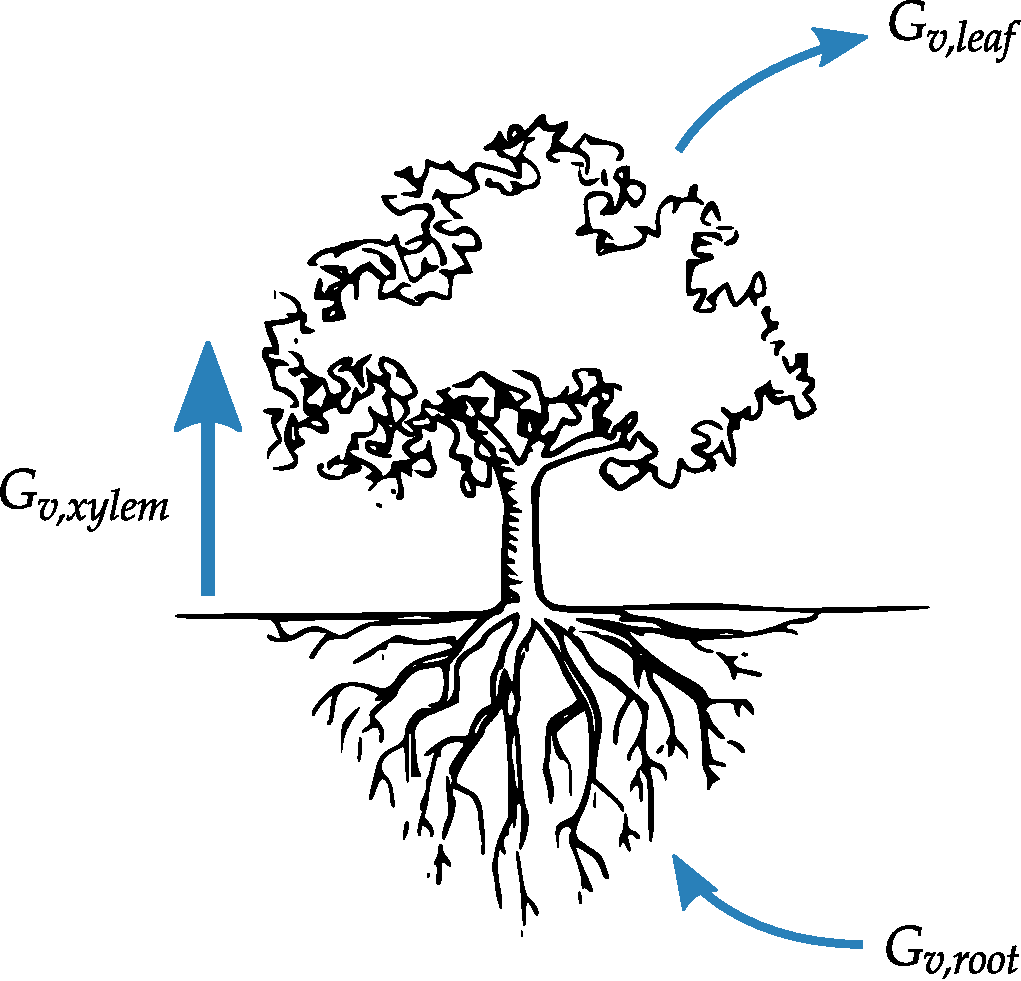
\includegraphics[width=0.5\textwidth]{\figdir/SPAC_waterbalance-crop.pdf}
	\caption{Soil-Plant-Atmosphere Continuum: The water balance between plant transpiration and root water uptake, $G_{\textit{v,root}} = G_{\textit{v,xylem}} = G_{\textit{v,leaf}}$.}
	\label{fig:SPAC_waterbalance}
\end{figure}

\subsection{Water transport in soil-root system}

The sink term $s_r$ (kg\,m$^{-3}$\,s$^{-1}$) due to root water uptake in soil moisture transport equation (\cref{eq:com6}) is simply defined as:
\begin{equation}
s_r = r \, g_{\textit{v,root}}
\end{equation}
where $r$ (m$^2$\,m$^{-3}$) is the root area density and $g_{\textit{v,root}}$ (kg\,m$^{-2}$\,s$^{-1}$) is the root water uptake, i.e., the flux of water from root to soil. It is defined as:
\begin{equation}
g_{\textit{v,root}} = k_{sr}^*\left(\psi_s - \psi_R\right)
\end{equation}
where $k_{sr}^*$ (s\,m$^{-1}$) is effective conductance of the soil-root system (i.e., rhizosphere), $\psi_s$ (Pa) is the soil water potential, and $\psi_R$ (Pa) is the (bulk) root water potential. The effective conductance of the soil-root system (or rhizosphere) $k_{sr}^*$ (s\,m$^{-1}$) is given as:
\begin{equation}
k_{sr}^* = \frac{1}{|\mvec{g}|} \frac{k_s\,k_r}{k_s + k_r}
\end{equation}
where $\mvec{g}$ (m\,s$^{-2}$) is the gravitational acceleration, $k_s$ (s$^{-1}$) is the soil conductance in the root region, and $k_r$ (s$^{-1}$) is the conductance of the root system. The soil conductance in the root region $k_s$ (s$^{-1}$) is defined as:
\begin{equation}
k_s = \alpha \, K \, r
\end{equation}
where
\begin{equation}
\alpha =  \sqrt{\left(\frac{L}{\textit{RAI}}\right) \frac{1}{d}}
\end{equation}
$d$ (m) is the root diameter, $L$ (m) is the root-depth height, and $\textit{RAI} = \int r\,\mathrm{d}z$ is the root area index (m$^2$\,m$^{-2}$). The hydraulic conductivity in soil $K$ (m\,s$^{-1}$) is given as:
\begin{equation}
K = K_{\textit{lp}} \, |\mvec{g}|
\end{equation}
where $K_{\textit{lp}}$ (s) being the liquid permeability defined in the \cref{subsec:ctoham}. Finally, the conductance of the root system $k_r$ (s$^{-1}$) is given as:
\begin{equation}
k_r = r \frac{\Delta z}{\beta}
\end{equation}
where $\Delta z$ is the vertical height of the root layer mesh and $\beta = \num{3e8}$ s. 

\begin{figure}[t]
	\centering
e
	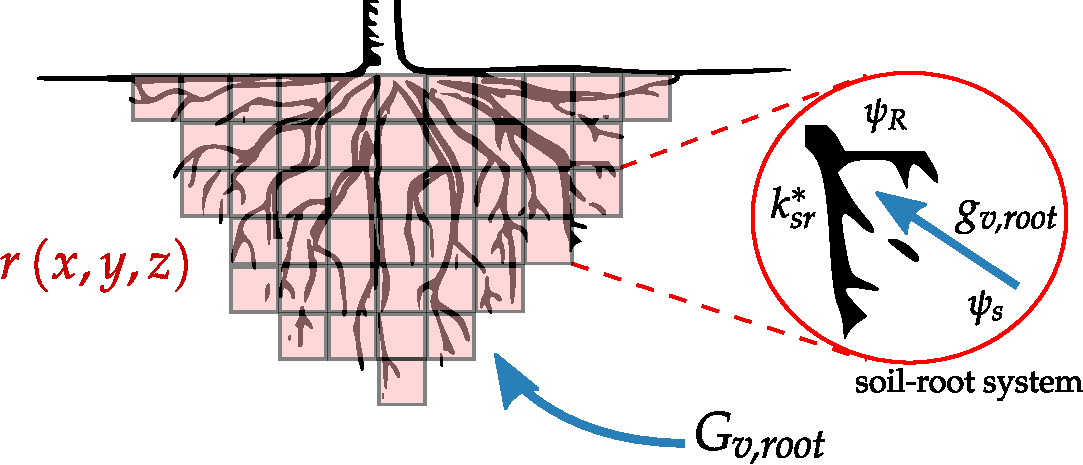
\includegraphics[width=0.65\textwidth]{\figdir/SPAC_root_v2-crop.pdf}
	\caption{Soil-Plant-Atmosphere Continuum: The water transport in soil-root system.}
	\label{fig:SPAC_root}
\end{figure}

Thus, the net root water uptake from the soil domain $G_{\textit{v,root}}$ (kg\,s$^{-1}$) is given as:
\begin{equation}
G_{\textit{v,root}} = \int_{\Omega_s} s_r\,\mathrm{d}V = \int_{\Omega_s} r\,g_{\textit{v,root}}\,\mathrm{d}V
\end{equation}
where $\Omega_s$ denotes the soil domain. 

%The water uptake from the root is equal to the water transport in the xylem as so:
%\begin{equation}
%G_{\textit{v,root}} = G_{\textit{v,xylem}}
%\end{equation}

\subsection{Water transport in xylem}

The water flux through the plant in xylem $g_{\textit{v,xylem}}$ (kg\,m$^{-2}$\,s$^{-1}$) is defined as:
\begin{equation}
g_{\textit{v,xylem}}(\psi_L) = k_x^* \left(\psi_R - \psi_L\right)
\end{equation}
where $k_x^*$ (s\,m$^{-1}$) is the effective xylem conductance, $\psi_R$ (Pa) is the (bulk) root water potential, and $\psi_L$ (Pa) is the (bulk) leaf water potential. The net water flux $G_{\textit{v,xylem}}$ (kg\,s$^{-1}$) is given as:
\begin{equation}   
G_{\textit{v,xylem}} = \int_{\partial\Omega_{x|s}} g_{\textit{v,xylem}}~\mathrm{d}A = g_{\textit{v,xylem}} A_x
\label{eq:netwaterflux_xylem}
\end{equation}
where $A_x$ (m$^2$) is the xylem cross-sectional area. The effective xylem conductance $k_x^*$ (s\,m$^{-1}$) of water is:
\begin{equation}
k_x^* = k_x \, \rho_l
\end{equation}
where plant xylem conductance $k_x$ (m\,Pa$^{-1}$\,s$^{-1}$) is modeled using a ``\textit{vulnerability curve}'' approach. The xylem conductance becomes exponentially smaller with increasing leaf water potential \citep{Volpe2013}. This empirical model is based on plant response to the vulnerability to xylem cavitation and embolism that could occur at high water potential gradients. The xylem conductance $k_x$ (m\,Pa$^{-1}$\,s$^{-1}$) is defined by:
\begin{equation}
k_x = k_{\textit{x,max}} \exp \left\{ - \left( - \frac{\psi_L}{d}\right)^c \right\}
\end{equation}
where $k_{\textit{x,max}}$ (m\,Pa$^{-1}$\,s$^{-1}$) is the maximum xylem conductance, and $c$ and $d$ are fit-coefficients \citep{Volpe2013}.


\begin{figure}[t]
	\centering
	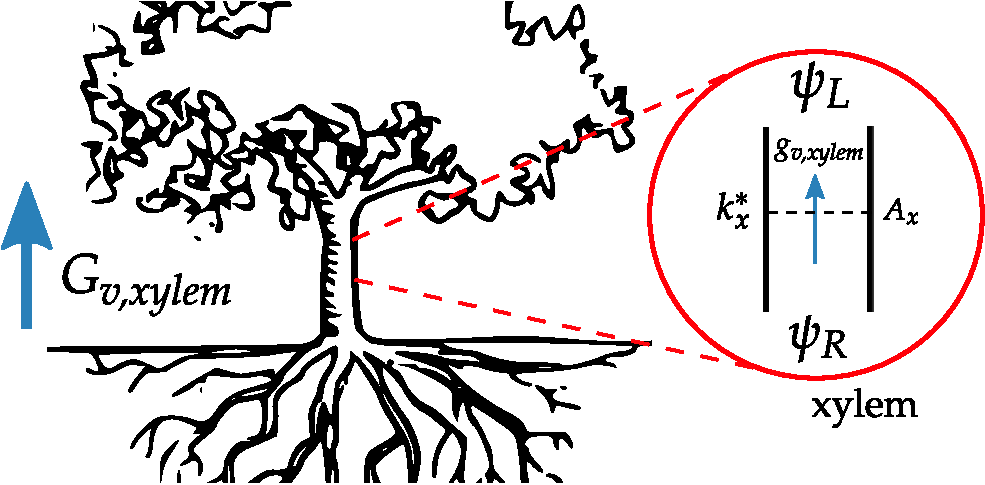
\includegraphics[width=0.65\textwidth]{\figdir/SPAC_xylem-crop.pdf}
	\caption{Soil-Plant-Atmosphere Continuum: The water transport in plant xylem.}
	\label{fig:SPAC_xylem}
\end{figure}

%Similarly, the net flux of water in xylem should be equal to the net transpiration rate, as storage is negligible. Therefore, 
%\begin{equation}
%G_{\textit{v,xylem}} = G_{\textit{v,leaf}}
%\end{equation}
%and moreover,
%\begin{equation}
%G_{\textit{v,root}}  = G_{\textit{v,xylem}} = G_{\textit{v,leaf}}
%\end{equation}

\subsection{Water transport from leaf to air}

The leaf transpiration rate $g_{\textit{v,leaf}}$ (kg\,m$^{-2}$s$^{-1}$) is defined in \cref{ch:parametricstudy}, and is simply defined as:
\begin{equation}
g_{\textit{v,leaf}} = k_{st,v}^* \left(\frac{p_{\textit{v,leaf}} - p_v}{p}\right)
\end{equation}
where $p_{\textit{v,leaf}}$ (Pa) is the vapor pressure at the leaf, $p_v$ (Pa) is the ambient vapor pressure, $p$ (Pa) is ambient pressure, and $k_{st,v}^*$ (kg\,m$^{-2}$\,s$^{-1}$) is the effective stomatal conductance to water vapor. It is defined as:
\begin{equation}
k_{\textit{st,v}}^* = M_w\,k_{\textit{st,v}}
\end{equation}
where $M_v = \num{1.8015e-2}$ kg\,mol$^{-1}$ is the molar mass of water vapor and $k_{\textit{st,v}}$ (mol$\,$m$^{-2}$$\,$s$^{-1}$) is the stomatal conductance to water vapor in molar units (the molar unit is commonly used in plant-science community). The stomatal conductance to water vapor is described in detail in \cref{subsec:sm}.

\begin{figure}[t]
	\centering
	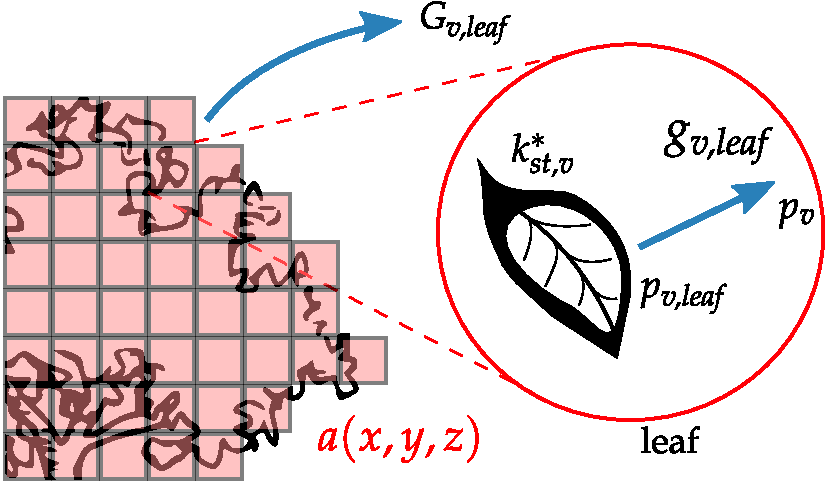
\includegraphics[width=0.65\textwidth]{\figdir/SPAC_leaf-crop.pdf}
	\caption{Soil-Plant-Atmosphere Continuum: The water transport from leaf to air.}
	\label{fig:SPAC_leaf}
\end{figure}

The net plant transpiration rate $G_{\textit{v,leaf}}$ (kg\,s$^{-1}$) is given as:
%The stomatal condutance is given as:
%\begin{equation}
%k_s = \frac{\rho}{p} \frac{R_a}{R_v} \frac{1}{r_a + r_s} 
%\end{equation}
%and so the net plant transpiration is given as:
\begin{equation}
G_{\textit{v,leaf}} = \int_{\Omega_a} a\,g_{\textit{v,leaf}}~\mathrm{d}V
\label{eq:netwaterflux_leaf}
\end{equation}
where $a$ (m$^2$\,m$^{-3}$) is the leaf area density and $\Omega_a$ denotes the air domain. As the water mass flux to the atmosphere is in equilibrium with the water vapor flux through xylem, i.e., as shown in \cref{eq:massfluxeq}, we can equate \cref{eq:netwaterflux_leaf} to \cref{eq:netwaterflux_xylem}:
\begin{equation}
G_{\textit{v,leaf}} = G_{\textit{v,xylem}}
\end{equation}
and so:
\begin{equation}
G_{\textit{v,leaf}} = k_x^* \left( \psi_R - \psi_L \right) A_x
\end{equation}
Therefore, we can determine the root water potential $\psi_R$ as follows:
\begin{equation}
\psi_R = \psi_L  + \frac{G_{\textit{v,leaf}}}{A_x k_x^*}
\end{equation}
and is simply dependent on the leaf water potential $\psi_L$ (Pa), the net plant transpiration rate $G_{\textit{v,leaf}}$ (kg\,s$^{-1}$), effective xylem conductance $k_x^*$ (s\,m$^{-1}$), and the xylem cross-sectional area $A_x$ (m$^2$). Additionally, we can also take in account of the influence of graviational potential change due to height of the plant as follows:
\begin{equation}
\psi_R = \psi_L  + \frac{G_{\textit{v,leaf}}}{A_x k_x^*} + \underbrace{\rho_l g H}_{\psi_g}
\end{equation}
For a plant with a plant canopy height of $H = 10$ m, the additional potential is $\psi_g = 0.1$ MPa and typically is negligible compared to the contribution of leaf water potential.


\subsection{Stomatal model with water stress sensitivity}
\label{subsec:sm}
	
The photosynthetic reaction creates carbohydrate and oxygen from light, water, and CO$_2$. Therefore, the photosynthetic rate $f_c$ (mol\,m$^{-2}$\,s$^{-1}$) defined as the rate of CO$_2$ assimilated by the plant (i.e., denoted also as $A_n$ (in plant-science) or $G_{\textit{c,leaf}}$ (in building physics), also known as assimilation rate) is directly related to atmospheric condition such as CO$_2$ concentration, availability of light and temperature. The assimilation rate is defined through Fickian diffusion law as:
The Fickian diffusion through stomata is given as:
\begin{equation}
f_c = k_{\textit{st}} \left(c_a - c_i\right)
\label{eq:fickassim}
\end{equation}
where $k_{st}$ (mol\,m$^{-2}$\,s$^{-1}$) is the (molar) stomatal condutance to CO$_2$ (note that for now we neglect the boundary layer conductance), $c_i$ (mol\,mol$^{-1}$) is the intercellular CO$_2$ concentration, and $c_a$ (mol\,mol$^{-1}$) is the ambient CO$_2$ concentration. However, during the opening of the stomata, additional moisture is lost by evaporation due to exposure of stomatal cavity to the atmosphere. Therefore, the transpiration rate $f_v$ (mol\,m$^{-2}$\,s$^{-1}$) (i.e. denoted also as $f_e$ (in plant-science) or $G_{\textit{v,leaf}}$ (in building physics), and also known as water use) is dependent on the atmospheric humidity and the availability of water for transpiration \citep{Ball1987,Leuning1995}. It is similarly described, based on Fickian diffusion process:
\begin{equation}
f_v = k_{\textit{st,v}} \left(\frac{p_{v,i} - p_v}{p}\right)
\label{eq:fv}
\end{equation}
where $k_{\textit{st,v}}$ (mol\,m$^{-2}$\,s$^{-1}$) is the (molar) stomatal condutance to water vapor, $p_{v,i}$ (Pa) is the intercellular vapor pressure, and $p_v$ (Pa) is the ambient vapor pressure. The water vapor stomatal conductance is related to the CO$_2$ stomatal condutance as:
\begin{equation}
k_{\textit{st,v}} = a_c \, k_{\textit{st}}
\end{equation}
where $a_c = 1.6$ is the relative diffusion of water vapor to CO$_2$. Furthermore, $p_{v,i} = p_{v,sat}\left(T_l\right)$ (Pa) where the intercellular vapor pressure inside the stomatal cavity is assumed to be at saturation at the leaf temperature $T_l$. 

So, the stomatal regulatory function is can be modeled through appropriate stomatal conductance. A generally accepted theory of plant response is that the plant regulates the stomatal aperature to optimize the photosynthetic rate for a given transpiration rate. Thus, the function of vegetation can be simplified as just maximizing the photosynthesis (or CO$_2$ assimilation) for a given transpiration rate (water use) \citep{Medlyn2011} and the water use efficiency (WUE) quantifies the efficiency of the plant of reaching this target:
\begin{equation}
\textit{WUE} = \frac{f_c}{f_v}
\label{eq:wue}
\end{equation}

The ``\textit{stomatal optimality model}'' reflects the theory of such stomatal behavior \citep{Cowan1978}. The optimal stomatal control is derived from the minimization problem described by the Lagrangian:
\begin{equation} 
\mathcal{L}(k_{st}) = f_c - \lambda f_v
\end{equation}
where $\lambda$ (mol\,mol$^{-1}$) is a Lagrange multiplier and represents the marginal water cost of plant carbon gain \citep{Medlyn2011,Katul2010,Manoli2014} and $f_c = f_c(k_{st})$ and $f_v=f_v(k_{st})$ are a function of stomatal conductance. \cite{Cowan1978} shows that optimal stomatal behaviour is at the minima of the Lagrangian:
\begin{equation}
\pde{\mathcal{L}}{k_{st}} = 0
\label{eq:lagrangian1}
\end{equation}
leading to the following constraint:
\begin{equation}
\lambda = \pde{f_v}{k_{st}}\pde{k_{st}}{f_c} 
\end{equation}
or simply:
\begin{equation}
\lambda = \pde{f_v}{f_c} 
\end{equation}

Following these constraints, the stomatal conductance $k_{\textit{st}}$ can be determined, given that unknowns in the assimilation rate $f_c$ are closed. To provide a closure for the assimilation rate, the assimilation rate $f_c$ described from the perspective of photochemical reaction model is also used. The Farquhar model of photosynthesis describing the biochemical demand function is given as:
\begin{equation}
f_c = \frac{a_1 c_i}{a_2 + s\,c_a}
\label{eq:bioassim}
\end{equation}
where $c_i$ (mol\,mol$^{-1}$)  is the intercellular CO$_2$ concentration, $c_a$ (mol\,mol$^{-1}$) is the ambient CO$_2$ concentration, and $a_1$ and $a_2$ are parameters dependent on whether photosynthetic reaction rate is limited by light or RuBisCO (Rubilose bisphosphate (RuBP) carboxylase-oxygenase) \citep{Katul2010, Farquhar1980}, and $s=0.7$ is the constant representing long-term intercellular to ambient CO$_2$ concentration ratio \citep{Volpe2013}. A detailed description of calculating $a_1$ and $a_2$ are given in \cref{subsubsec:ar}.

%Therefore,
%The Fickian diffusion through stomata is given as:
%\begin{align}
%f_c &= k_{\textit{st}} \left(c_a - c_i\right) \\
%f_v &= k_{\textit{st,v}} \left(\frac{p_{v,i} - p_v}{p}\right)
%\end{align}
%where $k_{\textit{st,v}}$ (mol\,m$^{-2}$\,s$^{-1}$) is the stomatal condutance to water vapor:
%\begin{equation}
%k_{\textit{st,v}} = a_c k_{\textit{st}} 
%\end{equation}
%where $a_c = 1.6$ is the relative diffusion of water vapor to CO$_2$. Furthermore, $p_{v,i} = p_{v,sat}\left(T_l\right)$ (Pa) is the intercellular vapor pressure inside the stomatal cavity assumed to be at saturation at the leaf temperature $T_l$. 

To solve for the stomatal conductance $k_{st}$, the remaining unknown is the intercellular CO$_2$ concentration $c_i$. We can determine this by equating Fickian CO$_2$ flux (\cref{eq:fickassim}) to the Farquhar biochemical demand (\cref{eq:bioassim}):
\begin{equation}
f_c = \frac{a_1\,c_i}{a_2 + s\,c_a} = k_{st} \left(c_a - c_i\right)
\end{equation}
and rewriting it for $c_i$, we get:
\begin{equation}
c_i = c_a \frac{a_2 + s\,c_a}{a_1/k_{st} + a_2 + s\,c_a}
\label{eq:ci}
\end{equation}
So, substituting \cref{eq:ci} back into the biochemical demand function (\cref{eq:bioassim}), the assimilation rate becomes a closed-problem:
\begin{equation}
f_c = \frac{k_{st}\,a_1\,c_a}{a_1 + k_{st} \left(a_2 + s\,c_a\right)}
\label{eq:fc2}
\end{equation}
where only the $k_{st}$ is the remaining unknown. Finally, the stomatal conductance $k_{\textit{st}}$ can be determined by solving \cref{eq:lagrangian1}:
\begin{equation}
\pde{\mathcal{L}}{k_{st}} = \pde{f_c}{k_{st}} - \lambda \pde{f_v}{k_{st}} = 0
\label{eq:lagrangian2}
\end{equation}
Substituting \cref{eq:fc2} and \cref{eq:fv} into \cref{eq:lagrangian2}, we have:
\begin{equation}
\pde{}{k_{st}} \left[ \left(\frac{k_{st}\, a_1 \,c_a}{a_1 + k_{st} \left(a_2 + s\, c_a\right)}\right)- \lambda\, a_c\, k_{\textit{st}}\, \textit{VPD} \right] = 0
\label{eq:lagrangian3}
\end{equation}
where $\textit{VPD} \equiv \left(p_{v,i} - p_v \right)/p$ (mol\,mol$^{-1}$). Solving \cref{eq:lagrangian3}, we get:
\begin{equation}
\frac{a_1^2\, c_a}{\left[a_1 + k_{st} \left(a_2 + s \,c_a\right)\right]^2}- \lambda\, a_c \,\textit{VPD} = 0
\end{equation}
and rewriting it for $k_{\textit{st}}$, we obtain:
\begin{equation}
k_{\textit{st}} = \frac{a_1}{a_2 + s\,c_a} \left( -1 + \sqrt{\frac{c_a}{a_c\, \lambda \,\textit{VPD}}} \right)
\label{eq:kst}
\end{equation}
Additionally, in literature it is known that stomata does not completely close during night allowing for respiration. Therefore, taking this into account:
\begin{equation}
k_{\textit{st}} = \frac{a_1}{a_2 + s\,c_a} \left( -1 + \sqrt{\frac{c_a}{a_c\, \lambda\, \textit{VPD}}} \right) + k_{\textit{st,n}}
\end{equation}
where $k_{\textit{st,n}}$ (mol\,m$^{-2}$\,s$^{-1}$) is the nocturnal stomatal conductance ($k_{\textit{st,n}} = 0.018$ mol\,m$^{-2}$\,s$^{-1}$, \citep{Manoli2014}). 

Thus, we obtain a stomatal model that is a function of the CO$_2$ assimilation (through parameters $a_1$, $a_2$ and $c_a$), atmospheric evaporative demand (AED) (through parameter $\textit{VPD}$), and the Lagrangian multipier $\lambda$ which represents the marginal water cost of plant carbon gain. Therefore, $\lambda$ reflects the sensitivity to water availability is also commonly known as the \textit{marginal water use efficiency}. It is empirically related to the leaf water potential $\lambda = \lambda(\psi_L)$ \citep{Manoli2014,Katul2010} and so, the stomatal response change to water availability is reflected through the change in leaf water potential $\psi_L$. The marginal WUE is determined from experimental measurements of plant photosynthesis, transpiration and stomatal conductance, and solving for the gradient of 
\cref{eq:wue}. An empirical model of marginal WUE, $\lambda$, as a function of leaf water potential $\psi_L$ \citep{Manoli2014,Katul2010}, is given as:
\begin{equation}
\lambda \left(\psi_L\right) = \lambda_{\textit{max}}^* \frac{c_a}{c_a^*}\exp \left\{-\beta \Big( \langle \psi_L \rangle_{\textit{24h}} - \psi_{\textit{L,max}}\Big)^2\right\}
\label{eq:mwue}
\end{equation}
where $\psi_L$ is assumed to vary slowly such that $\langle \psi_L \rangle_{\textit{24h}}$ is fixed within the secant iteration, $\lambda_{max}^*$ is the marginal WUE under well-watered soil condition at reference CO$_2$ concentration $c_a^*=400$ $\mu$mol~mol$^{-1}$ or parts-per-million (ppm), $\beta$ is the plant-specific sensitivity parameter \citep{Huang2017}.

Now that, we have closed $k_{\textit{st}}$ through \cref{eq:kst}, the intercellular CO$_2$ equation can be further simplified. Substituting \cref{eq:kst} into \cref{eq:ci}, it becomes:
\begin{equation}
c_i = \left(c_a - \sqrt{a_c\,\lambda\, \textit{VPD}\, c_a} \right)
\label{eq:ci2}
\end{equation}
meaning that it is only dependent on the ambient CO$_2$ concentration, vapor pressure deficit, and the marginal water use efficiency. Substituting \cref{eq:ci2} into \cref{eq:fc2}, gives:
\begin{equation}
f_c = \frac{a_1\,c_a}{a_2 + s\,c_a}\left(1-\sqrt{a_c\, \lambda\, \textit{VPD}\, c_a}\right)
\end{equation} 

%and thus closing the (with the exception of $\lambda$) the photosynthetic rate. So far, the stomatal conductance model is derived by neglecting the contribution of boundary layer conductance $k_{b}$ (i.e. $g_b$ (in plant-science), or inverse of boundary layer resistance $r_b$, assumed to be equivalent to aerodynamic resistance $r_a$). Therefore, the effective stomatal conductance $k_{st}^*$ is defined as:
%\begin{equation}
%k_{st}^* = \frac{k_{st} k_b}{k_{st} + k_b}
%\end{equation}
%assuming the resistance are in series. Therefore, the plant fluxes into atmosphere become:
%\begin{align}
%f_{c} &= k_{st}^* f_c \\
%f_{v} &= k_{st,v}^*  f_v
%\end{align}

Finally, the fluxes from leaves in units kg\,m$^{-2}$\,s$^{-1}$ can be simply determined as:
\begin{align}
g_{c,leaf} &= M_c f_c \\
g_{v,leaf} &= M_v f_v
\end{align}
where $M_c = \num{4.401e-2}$ kg\,mol$^{-1}$ and $M_v = \num{1.8015e-2}$ kg\,mol$^{-1}$ are the molar mass of CO$_2$ and water vapor, respectively. So far, the stomatal conductance model is derived by neglecting the contribution of boundary layer conductance $k_{b}$ (i.e. $g_b$ (in plant-science), or inverse of boundary layer resistance $r_b$, assumed to be equivalent to aerodynamic resistance $r_a$). Therefore, the effective stomatal conductance $k_{st}^*$ is defined as:
\begin{equation}
k_{st}^* = \frac{k_{st} k_b}{k_{st} + k_b}
\end{equation}
where $k_{st}$ is given by \cref{eq:kst} and $k_b$ is discussed in \cref{ch:parametricstudy}. Thus, the leaf fluxes become:
\begin{align}
g_{c,leaf} &= M_c\, k_{\textit{st}}^* \left(c_a - c_i \right) \\
g_{v,leaf} &= M_v\, k_{\textit{st,v}}^* \left(\frac{p_{\textit{v,i}} - p_v}{p}\right)
\end{align}

\subsection{Assimilation rate}
\label{subsubsec:ar}

As the photosynthesis can either be \textit{light-limited} or \textit{Rubisco-limited}, the true assimilation rate $f_c$ is given as:
\begin{equation}
f_c = \min \left(f_{c}^l, f_c^r\right) 
\end{equation}
where $f_c^l$ is the assimilated limited by light and $f_c^r$ is assimilation rate limited by RuBisCO. Note that it is also possible to incorporate the dark (or night) respiration and in that case $f_c = \min \left(f_c^l, f_c^r\right) - r_d$, but is not modeled in our study.
	
\subsubsection*{Light-limited}

If assimilation is \textit{light-limited}, $a_1$ and $a_2$ is defined as \citep{Manoli2014,Katul2010}:
\begin{equation}
a_1 = \underbrace{\alpha_p\, e_m}_{\gamma}\, Q_p
\label{eq:fcl_a1}
\end{equation}
and 
\begin{equation}
a_2 = 2\,c_p
\label{eq:fcl_a2}
\end{equation}
where $\alpha_p$ is the leaf absorptivity of photosynthetically active radiation (PAR), $e_m$ is the maximum quantum efficiency of the leaf, $\gamma = 0.015$ is the apparent quantum yield, $Q_p$ (mol\,m$^{-2}$\,s$^{-1}$) is the flux of incoming PAR, and $c_p$ (mol\,mol$^{-1}$) is the the CO$_2$ compensation point. The CO$_2$ compensation point is determined as:
\begin{equation}
c_p = \frac{K_c}{2\,K_o} C_{\textit{o,a}} \frac{k_o}{k_c}
\label{eq:cp}
\end{equation}
where $k_c = 2.5$ s$^{-1}$ and $k_o = 0.18 k_c$, and:
\begin{align}
K_c &= K_{c,25} \exp\left\{ \gamma_c \left(T_l - 298.15\right)\right\} \\
K_o &= K_{o,25} \exp\left\{ \gamma_o \left(T_l - 298.15\right)\right\}
\end{align}
are Michaelis constant for CO$_2$ and O$_2$ inhibition (referenced at $25$ $^{\circ}$C), and $C_{\textit{o,a}} = 0.21$ mol\,mol$^{-1}$ is the oxygen concentration in the atmosphere \citep{Farquhar1980}, with $K_{c,25} = \num{3e-3}$ mol\,mol$^{-1}$, and $K_{o,25} = 0.3$ mol\,mol$^{-1}$. Thus, substituting \cref{eq:cp} into \cref{eq:fcl_a2}, and  \cref{eq:fcl_a1,eq:fcl_a2} into \cref{eq:fc2}, we get the light-limited assimilation rate $f_c^l$ as:
\begin{equation}
f_c^l = \frac{\gamma\,Q_p\,c_i}{2\,c_p + s\,c_a}
\end{equation}

\subsubsection*{Rubisco-limited}

If the assimilation rate is \textit{Rubisco-limited}, $a_1$ and $a_2$ is defined as \citep{Manoli2014,Katul2010}:
\begin{equation}
a_1 = V_{\textit{cmax}}
\label{eq:fcr_a1}
\end{equation} 
and
\begin{equation}
a_2 = K_c \left(1 + \frac{C_{\textit{o,a}}}{K_o}\right)
\label{eq:fcr_a2}
\end{equation} 
where $V_{\textit{c,max}}$ is the maximum carboxylation capacity (referenced at $25$ $^{\circ}$C). The maximum carboxylation capacity is given as:
\begin{equation}
V_{\textit{cmax}} = V_{\textit{cmax,25}} \frac{ \exp\left\{ 0.088 \left(T_l - 298.15\right)\right\} }{1 + \exp\left\{0.29\left(T_l - 314.15\right)\right\} }
\end{equation}
where $T_l$ (K) is the leaf temperature, $V_{\textit{cmax,25}} = \num{5.9e-5}$ mol\,m$^{-2}$\,s$^{-1}$,
$\gamma_c = 0.074$, and $\gamma_o = 0.015$. Thus, substituting \cref{eq:fcr_a1,eq:fcr_a2} into \cref{eq:fc2}, the Rubsico-limited assimilation rate is given as:
\begin{equation}
f_c^r = \frac{V_{\textit{cmax}}\,c_i}{K_c \left(1 + \frac{C_{o,a}}{K_o}\right) + s\,c_a}
\end{equation}

%
%The Fickian diffusion through stomata is given as:
%\begin{align}
%f_c &= k_{\textit{st}} \left(c_a - c_i\right) \\
%f_v &= k_{\textit{st,v}} \left(\frac{p_{v,i} - p_v}{p}\right)
%\end{align}
%where $k_{\textit{st,v}}$ (mol\,m$^{-2}$\,s$^{-1}$) is the stomatal condutance to water vapor:
%\begin{equation}
%k_{\textit{st,v}} = a_c k_{\textit{st}} 
%\end{equation}
%where $a_c = 1.6$ is the relative diffusion of water vapor to CO$_2$. Furthermore, $p_{v,i} = p_{v,sat}\left(T_l\right)$ (Pa) is the intercellular vapor pressure inside the stomatal cavity assumed to be at saturation at the leaf temperature $T_l$. Thus, equating Fickian CO$_2$ flux to the Farquhar biochemical demand, we have:
%\begin{equation}
%f_c = \frac{a_1 c_i}{a_2 + s c_a} = k_{st} \left(c_a - c_i\right)
%\end{equation}
%where $c_i$ is the unknown. Rewriting, we get:
%\begin{equation}
%c_i = c_a \frac{a_2 + s c_a}{a_1/k_{st} + a_2 + s c_a}
%\end{equation}
%and substituting $c_i$ into the biochemical demand function, the assimilation rate is a closed-problem as:
%\begin{equation}
%f_c = \frac{k_{st} a_1 c_a}{a_1 + k_{st} \left(a_2 + s c_a\right)}
%\end{equation}
%
%Thus, the stomatal conductance can be finally obtained from the minimizing the problem:
%\begin{equation}
%\pde{\mathcal{L}}{k_{st}} = \pde{f_c}{k_{st}} - \lambda \pde{f_v}{k_{st}} = 0
%\end{equation}
%which becomes:
%\begin{equation}
%\pde{}{k_{st}} \left[ \left(\frac{k_{st} a_1 c_a}{a_1 + k_{st} \left(a_2 + s c_a\right)}\right)- \lambda a_c k_st \textit{VPD} \right] = 0
%\end{equation}
%where $\textit{VPD} = \left(p_{v,i} - p_v \right)/p$ (mol\,mol$^{-1}$). The derivative becomes:
%\begin{equation}
%\frac{a_1^2 c_a}{\left[a_1 + k_{st} \left(a_2 + s c_a\right)\right]^2}- \lambda a_c \textit{VPD} = 0
%\end{equation}
%
%Therefore, solving for $k_{\textit{st}}$ we obtain:
%\begin{equation}
%k_{\textit{st}}(\mvec{x}) = \frac{a_1(\mvec{x}) }{a_2(\mvec{x})  + s c_a(\mvec{x}) } \left( -1 + \sqrt{\frac{c_a(\mvec{x}) }{a_c \lambda(\psi_l)  VPD(\mvec{x}) }} \right)
%\end{equation}
%where the marginal water use is empirically related to the leaf water potential $\lambda = \lambda(\psi_l)$ \citep{Manoli2014,Katul2010}. Therefore, the stomatal response change to water availability is reflected through the change in leaf water potential $\psi_l$.  Additionally, in literature it is known that stomata does not completely close during night allowing for respiration. Therefore, taking this into account:
%\begin{equation}
%k_{\textit{st}}(\mvec{x}) = \frac{a_1(\mvec{x}) }{a_2(\mvec{x})  + s c_a(\mvec{x}) } \left( -1 + \sqrt{\frac{c_a(\mvec{x}) }{a_c \lambda(\psi_l)  VPD(\mvec{x}) }} \right) + k_{\textit{st,n}}
%\end{equation}
%where $k_{\textit{st,n}}$ (mol\,m$^{-2}$\,s$^{-1}$) is the nocturnal stomatal conductance ($k_{\textit{st,n}} = 0.018$ mol\,m$^{-2}$\,s$^{-1}$ \citep{Manoli2014}). The intercellular CO$_2$ concentration simplifies to:
%\begin{equation}
%c_i = c_a \left(1 - \sqrt{\frac{a \lambda \textit{VPD} }{c_a}} \right)
%\end{equation}
%and thus closing the (with the exception of $\lambda$) the photosynthetic rate. So far, the stomatal conductance model is derived by neglecting the contribution of boundary layer conductance $k_{b}$ (i.e. $g_b$ (in plant-science), or inverse of boundary layer resistance $r_b$, assumed to be equivalent to aerodynamic resistance $r_a$). Therefore, the effective stomatal conductance $k_{st}^*$ is defined as:
%\begin{equation}
%k_{st}^* = \frac{k_{st} k_b}{k_{st} + k_b}
%\end{equation}
%assuming the resistance are in series. Therefore, the plant fluxes into atmosphere become:
%\begin{align}
%	f_{c} &= k_{st}^* f_c \\
%	f_{v} &= k_{st,v}^*  f_v
%\end{align}
%Furthermore, the fluxes in units kg\,m$^{-2}$\,s$^{-1}$ can be simply determined as:
%\begin{align}
%g_{c,leaf} &= M_c f_c \\
%g_{v,leaf} &= M_v f_v
%\end{align}
%where $M_c = \num{4.401e-2}$ kg\,mol$^{-1}$ and $M_v = \num{1.8015e-2}$ kg\,mol$^{-1}$ are the molar mass of CO$_2$ and water vapor, respectively. 

%\subsection{Marginal water use}
%%The simplified effective stomatal conductance $k_{st,v}^*$ (s~m$^{-1}$) is defined in \cref{ch:parametricstudy} and is given as:
%%\begin{equation}
%%k_{st,v}^* = \frac{\rho}{p} \frac{R_a}{R_v} \frac{1}{r_a + r_s} 
%%\end{equation}
%%where $r_a$ (s~m$^{-1}$) and $r_s$ (s~m$^{-1}$) are aerodynamic and stomatal conductance respectively. The effective stomatal conductance can also be rewritten in the conductance form:
%%\begin{equation}
%%k_{st,v}^* = \frac{\rho}{p} a_c \frac{\tilde{k}_{st} \tilde{k}_{a}}{\tilde{k}_{st}+\tilde{k}_a} 
%%\end{equation}
%%?????? , check???
%%where $a_c = R_v/R_a$ and $\tilde{k}_{st}$ and $\tilde{k}_a$ are stomatal and aerodynamic condutance in non-standard unit of m~s$^{-1}$. The common notation used by plant scientist is mol~m$^{-2}$~s$^{-1}$, and is converted simply using:
%%\begin{equation}
%%k_{st} = \frac{M_w}{\rho} \tilde{k}_{st}
%%\end{equation} 
%%where $M_w$ (kg~mol$^{-1}$) is molar mass of water. Therefore, the more common form of effective stomatal conductance to water vapor is:
%%\begin{equation}
%%k_{st,v}^* = \frac{1}{p} M_w a_c \frac{k_{st} k_{a}}{k_{st}+k_a} 
%%\end{equation}
%%where $k_{\textit{st}}$ is the stomatal condutance of CO$_2$. A more advanced stomatal model, that can not only respond to atmospheric conditions such as radiation, humidity and temperature, we need a stomatal model that can respond to the water availability.
%%
%%he advanced model is derived from the stomtal optimility hypothesis of maximizing leaf-level gas exchange that follows the the lagrangian:
%%
%%
%%\begin{equation} 
%%\mathcal{L} = A_n - \lambda f_e
%%\end{equation}
%%such that the lagrange multiplier $\lambda$ is given as:
%%\begin{equation}
%%\pde{A_n}{k_{st}} = \lambda \pde{f_e}{k_{st}}
%%\end{equation}
%%and is typically referred to as t
%
%The marginal water use efficiency (WUE) $\lambda$ or the cost-parameter for the cost of water lost from leaves. 
%
%The marginal WUE should change over time depending on the water availability \cite{Manzoni2011}.  The marginal WUE is estimated from photosynthesis, transpiration and stomatal conductance measurement, obtained simply from the gradient of WUE:
%\begin{equation}
%\textit{WUE} = \frac{f_c}{f_v}
%\end{equation}
%
%The observations derive a marginal WUE as a function of leaf water potential $\psi_L$:
%\begin{equation}
%\lambda \left(\psi_L\right) = \lambda_{\textit{max}}^* \frac{c_a}{c_a^*}\exp \left\{-\beta \Big( \langle \psi_L \rangle_{\textit{24h}} - \psi_{\textit{L,max}}\Big)^2\right\}
%\label{eq:mWUE}
%\end{equation}
%where $\psi_L$ is assumed to vary slowly such that $\langle \psi_L \rangle_{\textit{24h}}$ is fixed within the secant iteration, $\lambda_{max}^*$ is the marginal WUE under well-watered soil condition at reference CO$_2$ concentration $c_a^*=400$ $\mu$mol~mol$^{-1}$ or parts-per-million (ppm), $\beta$ is the plant-specific sensitivity parameter \citep{Huang2017}.
%
%%
%%Thus, the stomatal model is dependent on the photosynthetically active radiation (PAR) $Q_p$ (mol~m$^{-2}$~$s^{-1}$), CO$_2$ concentration $c_a$ (mol~mol$^{-1}$), plant species specific water use efficiency and the humidity in the air (i.e. vapor pressure deficit $\textit{VPD}$ (mol~mol$^{-1}$)). The modified stomatal conductance is given as:
%%\begin{equation}
%%k_{\textit{st}}(\mvec{x},\ \psi_L)= \frac{a_1(\mvec{x})}{a_2(\mvec{x}) + s~c_a(\mvec{x})}\left(-1 + \left(\frac{c_a(\mvec{x})}{a~\lambda(\psi_L)~\textit{VPD}(\mvec{x})} \right)^{\frac{1}{2}}\right) + k_{\textit{st,n}}
%%\end{equation}
%%where $s=0.7$ is the constant representing long-term intercellular to ambient CO$_2$ concentration ratio \citep{Volpe2013}. The constant $a=1.6$ is the ratio of water vapor diffusivity to CO$_2$, and $a_1$ and $a_2$ depends if assimilation rate $A_n$ during photosynthesis is light-limited or Rubsico-limited, and $k_{\textit{st,n}}$ is the nocturnal stomatal conductance enabling plant respiration.
%%
%%
%%
%%
%%
%%\subsubsection*{Assimilation rate}
%%
%%To determine whether the assimilation rate is light-limiting or Rubisco-limiting, the limiting assimilation rate $A_n$ (mol~m$^{-2}$s$^{-1}$)is defined as:
%%\begin{equation}
%%A_n = \min \left(A_E, A_C\right)
%%\end{equation}
%%where $A_E$ is assimilation rate restricted by light-drive electron transport process, and $A_C$ is assimilation rate restricted by Rubisco (Rubilose bisphosphate (RuBP) carboxylase-oxygenase activity). 
%%
%%The assimilation rate based on photosynthesis-cFPGarbon reaction model is defined as:
%%\begin{equation}
%%A_n(\mvec{x}) = \frac{a_1(\mvec{x}) \left(c_p(\mvec{x}) - c_i(\mvec{x})\right)}{a_2(\mvec{x}) + c_i(\mvec{x})}
%%\end{equation}
%%where $c_i$ is the intercellular CO$_2$ concentration. The assimilation rate is closed by relating the photochemical reaction model to the Fickian diffusion at the leaf surface:
%%\begin{equation}
%%A_n(\mvec{x}) = k_c^* \left(c_i(\mvec{x}) - c(\mvec{x})\right)
%%\end{equation} 
%%where $k_c^*$ is the stomatal conductance to CO$_2$ and $c$ is the atmospheric CO$_2$ concentration. Thus, the assimilation rate $A_n$ can be computed once the intercellular CO$_2$ concentration is known:
%%\begin{equation}
%%c_i = - \frac{1}{2} \left(\frac{a_1}{k_c^*} + a_2 - c \right) \pm \frac{1}{2}\sqrt{ \left(\frac{a_1}{k_c^*} + a_2 - c \right)^2 - 4\left(-\frac{a_1 c_{\textit{cp}}}{k_c^*} - c~a_2\right)}
%%\end{equation}
%%
%%The CO$_2$ conductance $k_{\textit{st,c}}$ (mol~m$^{-2}$\ s$^{-1}$) (molar) is given as:
%%\begin{equation}
%%k_{\textit{st,c}}^* = \frac{k_{\textit{st}}~k_a}{k_{\textit{st}} + k_a}
%%\end{equation}
%%where $k_{\textit{st}}$ (mol~m$^{-2}$~s$^{-1}$) is the (molar) stomatal conductance to CO$_2$, $k_a$ (mol~m$^{-2}$s$^{-1}$)  is the boundary layer conductance. The water vapor conductance is given as:
%%\begin{equation}
%%k_{\textit{st,v}}^* = a_c~k_{\textit{st,c}}^*
%%\end{equation}
%%where $a_c$ is the ratio of water vapor to CO$_2$ diffusion. The net water transport through xylem $G_{\textit{v,xylem}}$ (kg~s$^{-1}$) is given as:
%%\begin{equation}
%%G_{\textit{v,xylem}}\left(\psi_L\right) = k_x \left(\psi_R - \psi_L\right) \frac{A_x}{|\mvec{g}|} 
%%\end{equation}
%%where $k_x$ (s$^{-1}$) is the xylem conductance, $\psi_R$ is the root water potential and $\psi_l$ is the leaf water potential. 


\subsection{Numerical strategy for solving leaf water potential}

The water transport through the plant from soil to root, from root to xylem, through the xylem, and finally, from leaf stomata to air is a closed-problem once the leaf water potential is known. The leaf water potential is determined from \cref{eq:massfluxeq}:
\begin{equation}
G_{v,leaf}(\psi_L) = G_{v,root} (\psi_L)
\end{equation}

As an optimization problem, it is defined as:
\begin{equation}
\mathop {\mathrm{arg\ min} }\limits_{\psi_L}~\mathcal{G}(\psi _L) = \left| {{G_{\textit{v,leaf}}} - {G_{\textit{v,root}}}} \right|
\end{equation}

As this is a non-linear closure problem \citep{Manoli2014},  a secant method is employed to iteratively converge to the leaf water potential. The $j+1^\mathrm{th}$ leaf water potential estimate is determined as:
\begin{equation}
\psi_L^{j+1} = \psi_L^{j} - G(\psi_L^j) \frac{\psi_L^j - \psi_L^{j-1}}{G\left(\psi_L^j\right) - G\left(\psi_L^{j-1}\right) }
\end{equation}
where the initial estimate of $\psi_L^{j=0} = 0$ MPa and $\psi_L^{j=1} = -10$ MPa and with the additional constraint that $-10 \le \psi_L \le 0$ MPa, enforcing that leaf water potential is negative and not larger than $-10$ MPa. The detailed solution strategy for determining for coupling all the models is detailed in next section.

\section{Radiation model}
\label{sec:radiationmodel}
The radiative exchanges are summarized in this section.

%The numerical model for air domain, solid domains (soil, ground, building), the radiation model and the vegetation model is implemented into OpenFOAM. The solid and air domains are coupled at regular intervals $t^m$ defined as exchange timesteps or air time steps \citep{Saneinejad2014,Kubilay2018}. The fluxes between air and solid domain consisting for thermal, moisture and radiative transfers are coupled at this step, chosen to be 10 min. At each $t^m$, the air domain is assumed to the quasi-steady and solving using steady-state RANS approach converged when residuals of $\rho$, $\mvec{u}$, $h$, $k$, $\varepsilon$ are below threshold. During the steady-state computation, the leaf energy balance is evaluated periodically to correct the heat and mass fluxes, $q_{\textit{sen,leaf}}$ and $g_{\textit{v,leaf}}$, respectively. 

\section{Coupling algorithm}
\label{sec:couplingalgorithm}

The numerical models for air domain, solid domains (soil, ground, building facade), the radiation model and the vegetation model are implemented into OpenFOAM. \cref{fig:coupling} shows the schematic representation of the solid and air domain coupling strategy. The solid and air domains are coupled at regular intervals $t^m$ defined as exchange timesteps or air time steps \citep{Saneinejad2014,Kubilay2018}. The fluxes between air and solid domain consisting of thermal, moisture and radiative transfers are coupled at exchange timesteps, chosen to be an interval of $\Delta t^m = 10$ min.

\begin{figure}[t]
	\centering
	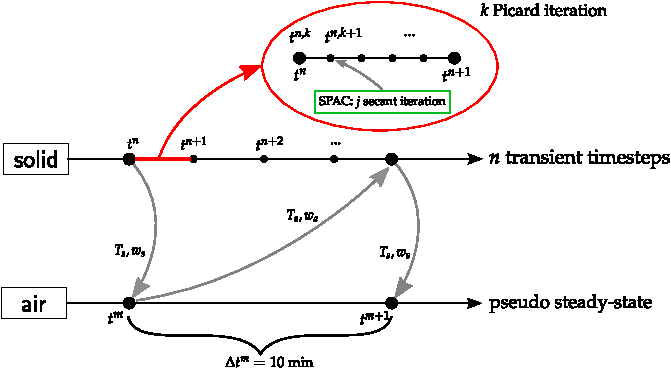
\includegraphics[width=\textwidth]{\figdir/coupling-crop.pdf}
	\caption{Schematic representation of the coupling strategy.}
	\label{fig:coupling}
\end{figure}


\subsection{Air domain}

The air domain is solved using $m$ pseudo steady-state timestep, discretizing the diurnal cycle of a day into $\num{8640}$ pseudo steady-state timesteps of $\Delta t^m = 10$ min (i.e., $8640$ time steps in a $24$ hrs). At each $m^{\mathrm{th}}$ step, a steady-state RANS model is solved for the fluid equations: $\rho$, $\mvec{u}$, $h$, $k$, and $\varepsilon$. During the steady-state computation, the \textit{leaf energy balance} (LEB) model is solved to determine the heat and mass fluxes, $q_{\textit{sen,leaf}}$ and $g_{\textit{v,leaf}}$, respectively. The algorithm for solving the air domain from $t^{m}\rightarrow t^{m+1}$ (as shown in \cref{fig:coupling}) is as follows:
\begin{enumerate}
	\item Update the radiation fields in the air domain using $q_{\textit{rad}}$ from building surfaces and determined $q_{\textit{r,lw}}$ and $q_{\textit{r,sw}}$.
	\item Solve \textit{leaf energy balance} (LEB) model:
	\begin{enumerate}
		\item Calculate radiative flux $q_{\mathit{rad,leaf}}$ using \cref{eq:qradleaf}.
		\item Calculate the stomatal and aerodynamic resistances $r_{s}$ and $r_{a}$ using \cref{eq:ra} and \cref{eq:rs}, respectively.
		\item Perform an initial estimate of leaf temperature $T_{\mathit{leaf}}=T$.
		\item Calculate saturated vapor pressure at the leaf surface $p_{\mathit{vsat,leaf}}=f(T_{\mathit{leaf}})$.
		\item Calculate latent heat flux $q_{\mathit{lat,leaf}}$ using \cref{eq:latentheatflux}. 
		\item Correct leaf temperature $T_{\mathit{leaf}}$ using \cref{eq:solveleaft}.
		\item Repeat steps (d) to (f) until the leaf temperature has converged ($\epsilon < \num{e-8}$).
	\end{enumerate}
	\item Calculate all vegetation source terms $s_\rho$, $\mvec{s}_u$, $s_T$, $s_w$, $s_k$ and $s_{\varepsilon}$ using \cref{eq:source_density,eq:source_mom,eq:source_temp,eq:source_humi,eq:source_k,eq:source_eps}.
	\item Solve for the steady-state airflow field for $t^{m+1}$, \crefrange{eq:conservationeq_incompressible1}{eq:conservationeq_incompressible6}.
	\item Repeat steps (2) to (4) until residuals of \crefrange{eq:conservationeq_incompressible1}{eq:conservationeq_incompressible6} have reached the convergence limit of $\epsilon < \num{e-6}$.
\end{enumerate}

\subsection{Solid domain}

The solid domain describes the heat and mass transport in urban structures such as building facade, pavement, road and the ground (i.e., soil). Each of these ``\textit{sub}'' domains consists of $n$ adaptive solid timesteps with $\Delta t^n < \Delta t^m$ as shown in \cref{fig:coupling} \citep{Kubilay2018,Janssen2002}. At the beginning of the solid domain iteration, the thermal, moisture and radiative transfers are updated providing the necessary boundary conditions for wall boundaries. For each of $n$ solid timesteps, the linearized heat and mass transport equation are solved using $k$ Picard iterations. In the soil sub-domain only, during each of these $k$ Picard iteration, the soil-plant-atmosphere continuum (SPAC) model is solved using $j$ secant iterations to determine the root water uptake \citep{Manoli2014}. The algorithm for solving such soil sub-domain is given as:
\begin{enumerate}
	\item $k$ Picard iterations solving for the linearized heat and mass transport transport equations:
		\begin{enumerate}[label=(\alph*)]
			\item Calculate marginal WUE $\lambda$. % As $\psi_L$ is assumed to be slowly varying, $\lambda$ is constant in secant iteration.
			\item Calculate stomatal conductance $k_{\textit{st}}$.
			\item Calculate assimilation rate $f_c$ and transpiration rate $f_v$.
			\item Calculate net transpiration rate $G_{\textit{v,leaf}}$.
			\item Calculate effective soil-root conductance $k_{sr}^*$.
			\item $j$ secant iterations solve for leaf water potential $\psi_L$.
				\begin{enumerate}[label=(\alph*)]
					\item Initial guess of leaf water potential, $\psi_L^{j=0} = 0$ MPa, $\psi_L^{j=1} = -10$ MPa.
					\item Calculate effective xylem conductance $k_x^*$.
					\item Calculate root water potential $\psi_R^j$.
					\item Calculate root uptake $g_{\textit{v,root}}$ and net root uptake $G_{\textit{v,root}}$.
					\item Calculate cost function $\mathcal{G}$.
					\item Correct leaf water potential using secant method $\psi_L^{j}\rightarrow\psi_L^{j+1}$.
					\item Repeat till leaf water potential is converged, $\delta \psi_L \le \epsilon$.
				\end{enumerate}
			\item Calculate the sink in soil moisture due to root water uptake $s_{r}$.
			\item Solve linearized form of heat and mass equation using PCG until $\delta p_c \le \num{e-2} $ and $\delta T \le  \num{e-2}$, repeating steps before.
		\end{enumerate}
	\item Use the final surface temperature $T_s^{N}$ to update $q_{\textit{r,lw}}$ fluxes at all surfaces.
	\item Final surface temperature $T_s^N$ and moisture fluxes $g_{v}^N$ are boundary conditions for the air domain at the following timestep $t^{m+1}$.
\end{enumerate}
